\part{Câmera e HUD}

\section{Câmera}

    A câmera do jogo será movimentada de acordo com a movimentação do mouse, de maneira que ao decorrer do percurso, o carro será mantido centralizado na tela, ou seja, passando a ser uma visão em terceira pessoa em diagonal.

\section{HUD}

    \subsection{Vida}

        Será disponibilizado uma vida ao jogador para cada tentativa não havendo nenhum tipo de energia. O jogador saiu da pista ou a gasolina acabou, a corrida esta encerrada.

    \subsection{Pontuação e Rankings}

        Para cada objeto coletado em jogo, o jogador sera bonificado com a pontuação definida na tabela do documento de visão. Ao final de cada percurso, o sistema fará a totalização da pontuação adquirida ao longo de toda da corrida e guardará o tempo totalizado marcado pelo jogador, para então realizar a atualização desses números na tabela de ranking local do sistema. Terão duas tabelas, a primeira será construida com base nos melhores tempos realizados naquela máquina e a segunda será por pontuação adquirida em jogo, e disposição dos nomes dos jogadores nas tabelas será do menor tempo para o maior e da maior pontuação para a menor. A pontuação será mostrada na parte inferior no canto esquerdo da tela.
        
    \subsection{Combustível}

        A barra de combustível do veículo ficará parte superior à esquerda na tela para que o jogador tenha noção da quantidade que resta para perder a tentativa. Ela será um barra horizontal divida em 3 secções onde quanto mais cheia, ela fica mais esverdeada e quanto mais vazia, ela fica avermelhada.

    \subsection{Tempo}

        O tempo de jogo será baseado no tempo que o jogador permanecer em corrida, enquanto ele se mantiver na pista entre a linha de chegada e a linha de partida, o jogo permanecerá rodando o relógio no canto superior direito.

    \subsection{Medidor de velocidade}

        Na tela da corrida haverá um medidor de velocidade parte inferior à direita na tela. \\\
        
\begin{figure}[!h]
		\centering
	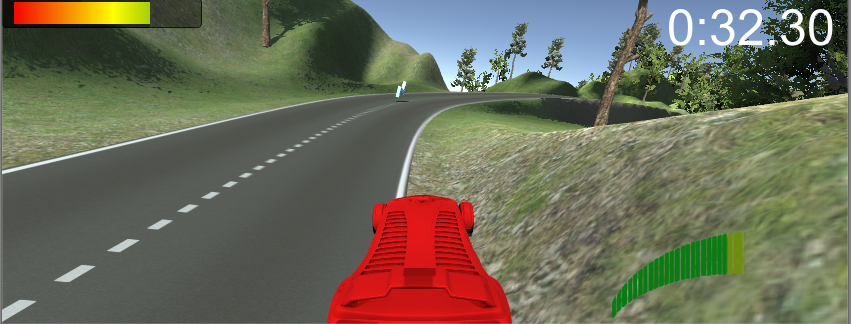
\includegraphics[scale=0.5]{figuras/hud}
		\caption{Tela de jogo}
\end{figure}

	\subsection{Mapa do Jogo}
	
\begin{figure}[!h]
		\centering
	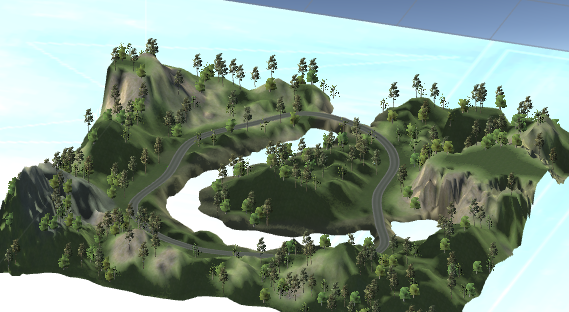
\includegraphics[scale=0.5]{figuras/mapa}
		\caption{Mapa geral do jogo}
\end{figure}	